\documentclass[titlepage]{article}

\usepackage[margin=1in]{geometry}
% some more shit for the title
\usepackage[T1]{fontenc}
\usepackage{babel}

% Tables and stopping them from displaying in a different section
\usepackage{booktabs}
\usepackage[section]{placeins}

% for inserting images into the document, setting file path, and allowing rotation of inserted images 
\usepackage{graphicx}
\graphicspath{ {./images/} }
\usepackage{rotating}
\usepackage[table]{xcolor}
% mostly just for putting text in math equations
\usepackage{amsmath}
% for aligning the text to the left
\usepackage[document]{ragged2e}

% for inserting hyperlinks in the document, use \url{url} or \href{url}{text}
\usepackage{hyperref}
\usepackage{calligra}
\usepackage[T1]{fontenc}
\usepackage{siunitx}
\usepackage{caption}
\usepackage{multirow}
\usepackage[export]{adjustbox}
\usepackage{tikz}
\usepackage{pgfplots}
\pgfplotsset{soldot/.style={color=black,only marks,mark=*},
	             holdot/.style={color=black,fill=white,only marks,mark=*},
		                  compat=1.12}
\usepackage{paracol}

\begin{document}
\title{\textbf{Lab 4: Resistivity of Nickel Chromium Wire and Use of the Wheatstone Bridge Circuit}}
\author{
    Zachary Pouska\\
    \texttt{001103193}\\
    \and
    Natalie Tran \\ 
    \texttt{000698629}\\ \\
    \and
    Joseph Pancho\\
    \texttt{002550975} \\ \\
} 

\date{PHYS 236 | Fall 2022\\
Date performed: 10/10/2022}


	\maketitle



	\section{Purpose}
    

	\section{Theory}	


	\section{Experiment Analysis}
        
        \subsection{Measurement of the resistivity $\rho$} 




    In part 1, our objective is to measure the resistivity constant of our nichrome wire. We can use the following equations to calculate the resistivity:
    $$\rho = R \frac{a}{l} \text{ where } A=\pi r^2$$ 
    $$ R=\rho \frac{l}{A} = \rho \frac{l}{\pi r^2}  \text{ in this case, R is a function of $\rho$, $l$, and $r$} $$

    Having used these equations, we found that the resistance of the wire, $R$, was 7.4$\Omega$, and the resistivity of the wire was equal to $(7.4)\frac{\pi \cdot (0.227 \cdot 10^{-3})^2}{1.0m} = 1.199\cdot 10^{-6}$. 

    The \textbf{uncertainty} of our measurement of the resistance was determined using the formula $$\Delta f= \frac{\partial f}{\partial x} \Delta x + \frac{\partial f}{\partial y} \Delta y + \frac{\partial f}{\partial z} \Delta z$$ for a function $f(x,y,z)$.
    Substituting in our values, we obtain the equation:
    $$\Delta R= \frac{\partial R}{\partial \rho} \Delta \rho + \frac{\partial R}{\partial l} \Delta y + \left|\frac{\partial R}{\partial r}\right| \Delta r$$ 
    Where $\partial \rho = \frac{l}{\pi r^2}$, $\Delta \rho = \text{range}$, $\partial l = \frac{\rho}{\pi r^2}$, $\Delta l =\text{resolution of meter stick + standard deviation of measurements}$, $\partial r = \frac{\rho l}{\pi}\cdot \frac{-2}{r^3}$ 
    
    


        \subsection{Part 2} 
        In a Wheatstone bridge, the wire connecting the two parallel resistors will have a point where the potential is 0 relative to the two pairs of series resistors, or in our case the point between our resistor box and the unknown resistor. In our setup, the nichrome wire is acting as our upper two resistors of a Wheatstone bridge, as it is divided essentially into two resistors. Using this phenomenon, we can "calibrate" the Wheatstone bridge by moving the point of contact across the nichrome wire, which then lets us assume that the points $P_1$ and $P_2$ have equal electric potentials. 

        \FloatBarrier
        \begin{figure}[hbt!] 
            \centering 
            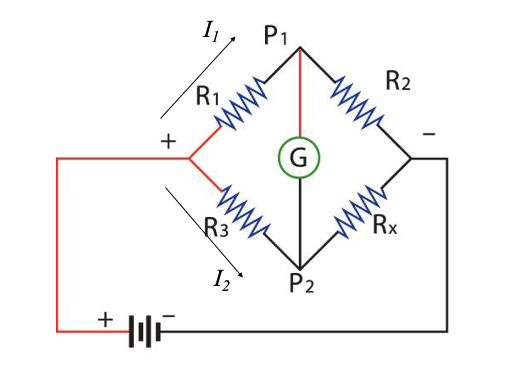
\includegraphics[scale = 0.4]{exanal/wheatstone}
        \end{figure}
        \FloatBarrier

        Then applying Kirchhoff's law from point $P_2$ to point $P_1$ travelling clockwise, we get $$V_{P2}+I_2 R_3 - I_1 R_1  V_{P1} $$ 
        $$ V_{P2} - V_{P1} = I_1 R_1 - I_2 R_3 $$
        and $$ I_1 R_1 = I_2 R_3$$
        Then traveling counter-clockwise, we get $$V_{P2}-I_2 R_x + I_1 R_2 = V_{P1} $$
        $$ V_{P2} - V_{P1} = I_2 R_x - I_1 R_2 = 0V $$
        $$I_2 R_x = I_1 R_2 $$
        and $$\frac{R_1}{R_2} = \frac{R_3}{R_x} $$ which can be further solved for $R_x$, giving us 
        $$R_x = \frac{R_s R_2}{R_1} $$
        where $R_s$ is our known standard resistor box. 

        Substituting our proportional values for $R_1$ and $R_2$ gives us $$R_x = \frac{R_s \left( \frac{\rho L_2}{A} \right)}{\left( \frac{\rho L_1}{A}  \right)} $$ But can still be further simplified to $$R_x=\frac{R_s L_2}{L_1} $$
since the values of the resistances are directly proportional to the lengths of each side of the wire (all other variables like the area and resistivity are held constant). 





	\section{Procedure}




	\section{Data and Graphs}
	\subsection{Part 1}
	\subsection{Part 2} 
	\subsection{Part 3}
	\section{Results}

	\section{Conclusion}

\end{document}
